\section{Synthetic CP data}

Equation \ref{eq1} is a general decomposition for matrices which are a distinct case of tensors. Tensor is a multidimensional matrix which its order is defined via the number of dimensions. A scalar value is a zero order tensor, an array is a first order tensor, a matrix is a second order tensor and then there are third fourth order tensor without no limit in the number of dimensions. 
The difference between matrix and tensor are:

\begin{itemize}
    \item Computing the rank of matrix is via SVD very straightforward whereas for the tensor it is a NP-hard.
    \item The rank of the tensor is different from its dimension whereas this is not the case for matrix which it 
\end{itemize}

Equation \ref{eq1} could be rewritten in terms of tensor product as below.


\begin{equation}\label{eq44}
    X=\sum_{k=1}^{R}\lambda_{r}a_{r}b_{r}+e=\sum_{k=1}^{R}\lambda_{r}a_{r}\circ b_{r}+e
\end{equation}

where $\circ$ is the outer product of the matrices and the product $a_{r}\circ b_{r}$ is a dyadic product of rank-1 matrices. Consequently a tensor is rank one only if it could be written as an outer product of N vectors, 

\begin{equation}
    X=a^{(1)}\circ a^{(2)}\cdots a^{(N)}
\end{equation}
whereby the tensor $X=a^{(1)}\circ a^{(2)}\circ a^{(3)}$ is a third order rank one. 
Decomposition in equation \ref{eq44} is extended into polydiac decomposition when the linear combination of rank-1 tensor in equation \ref{eq45}:

\begin{equation}\label{eq45}
    X=\sum_{k=1}^{R}\lambda_{r}b_{r}\circ b_{r}\cdots b_{r}+e
\end{equation}



The tensor rank is the minimum value R which equation \ref{eq45} sustain the equality. In case the decomposition is performed via the minimum number of rank-1 tensors this is called canonical polydiac decomposition CPD. The main advantage of CPD is the uniqueness of the decomposition without imposing specific constrain (c.f orthogonality and triangularity) as in the matrix case.  

A synthetic tensor T is being utilized for this study. Where its respective components A,B, and C ($T=\sum_{k=1}^{3}a_{r}\circ b_{r}\circ c_{R}+e$) are plotted in figure \ref{A},\ref{B} and \ref{C}.


\begin{figure}[!htbp]
\minipage{0.33\textwidth}%
\centering
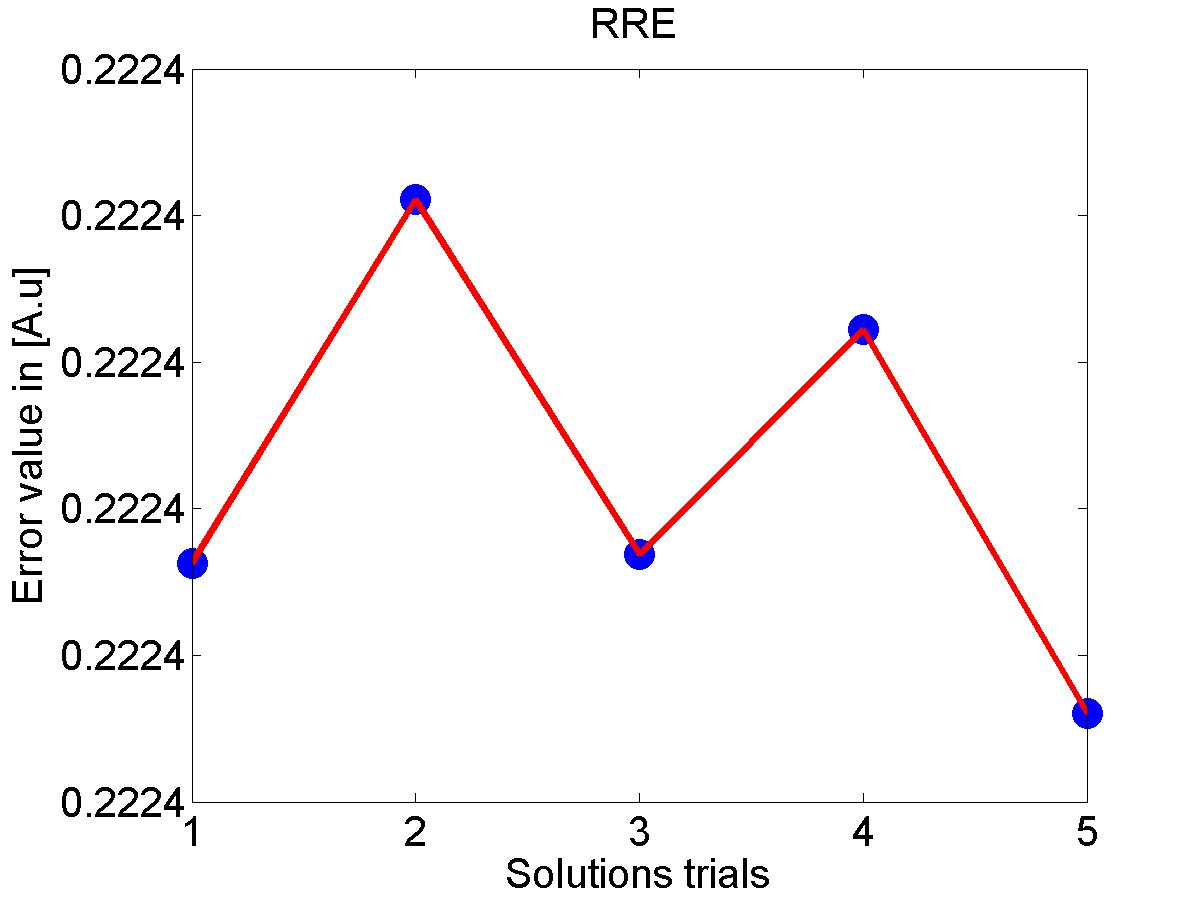
\includegraphics[width=1\linewidth]{201.jpg}
\subcaption{Component A}\label{A}
\endminipage\hfill
\minipage{0.33\textwidth}%
\centering
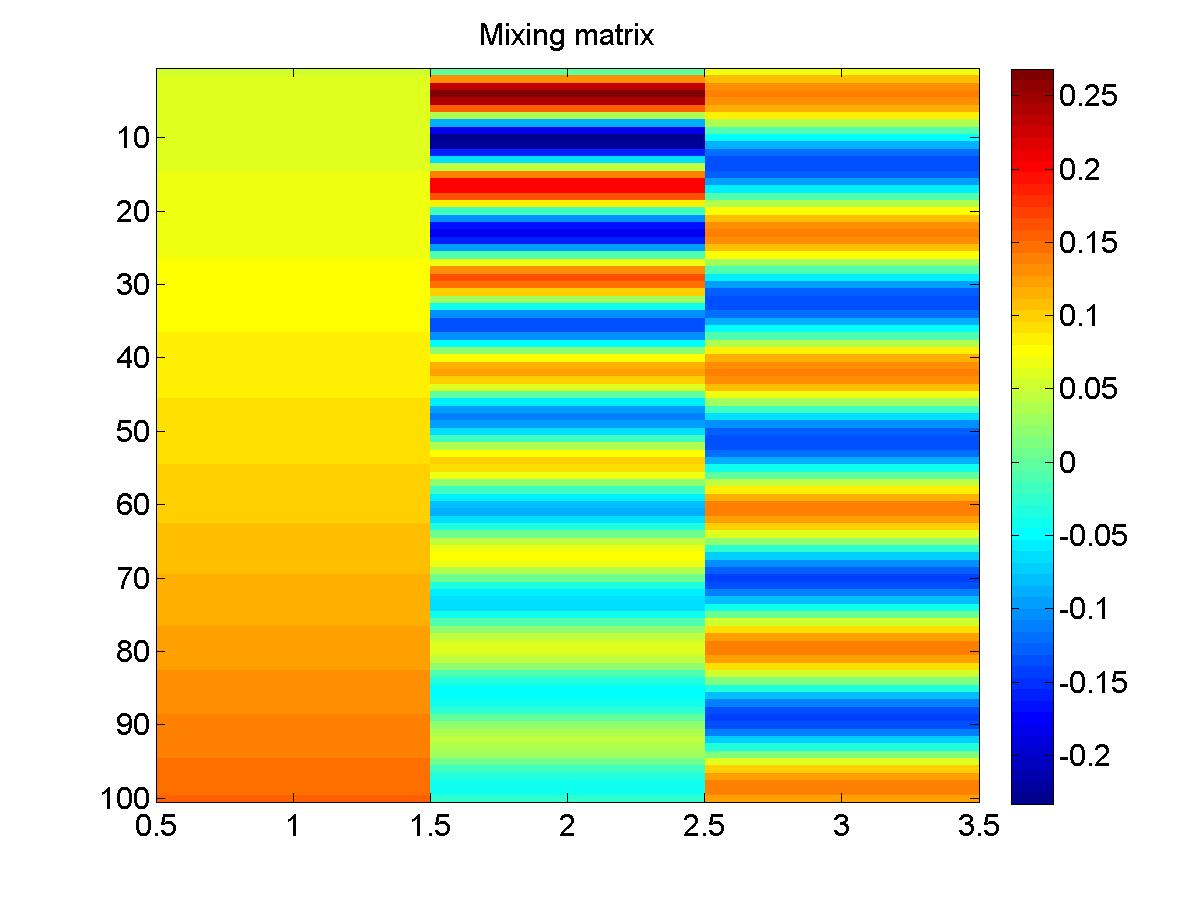
\includegraphics[width=1\linewidth]{202.jpg}
\subcaption{Component B}\label{B}
\endminipage\hfill
\minipage{0.33\textwidth}%
\centering
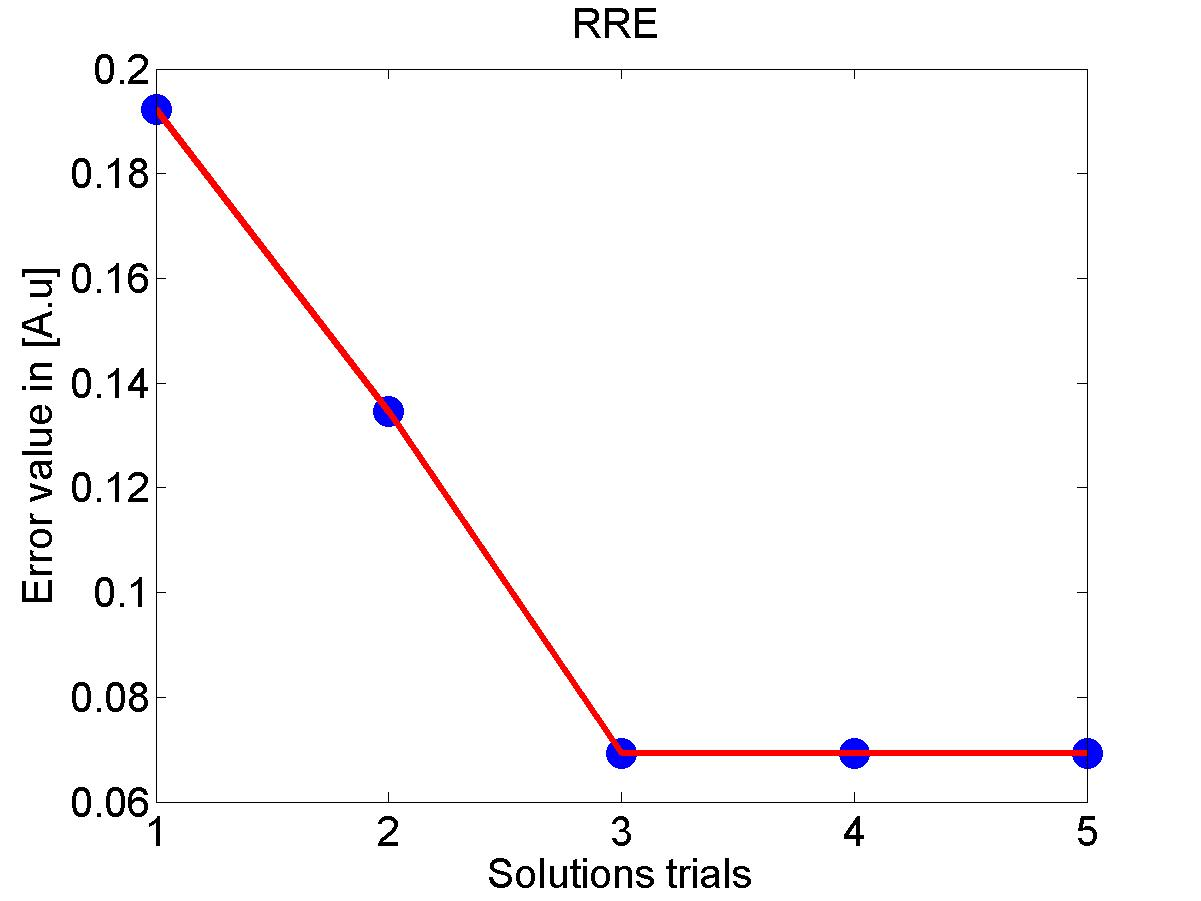
\includegraphics[width=1\linewidth]{203.jpg}
\subcaption{Component C}\label{C}
\endminipage\hfill
\caption{CPD of the tensor T}
\end{figure}

This matrices are respectively the mixing matrix figure \ref{A}, source matrices \ref{B} and the scaling matrix \ref{C}. 

Hereby the last component $T(:,:,4)$ figure \ref{T} will be decomposed via PCA and ICA in order to obtain the equivalent matrix of A,B and C which are respectively in figure \ref{EA}, \ref{EB} and  \ref{EC}. Alternatively ICA could also provide the mixing the the source signals but not the scaling matrix. The results for ICA are outlined in figure \ref{ICA_E}

\begin{figure}[!htbp]
\centering
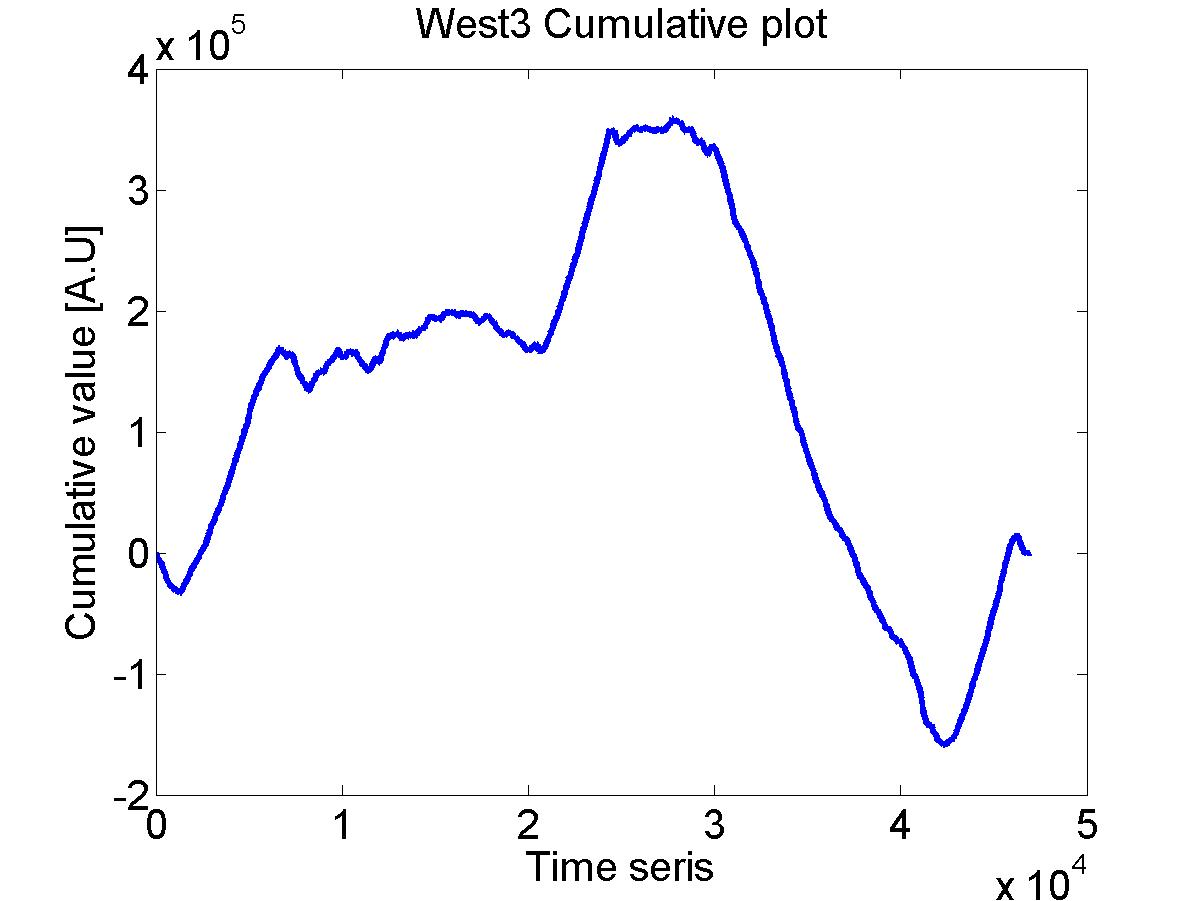
\includegraphics[width=0.5\linewidth]{200.jpg}
\caption{$T(:,:,4)$  component.}\label{T}
\end{figure}



\begin{figure}[!htbp]
\minipage{0.33\textwidth}%
\centering
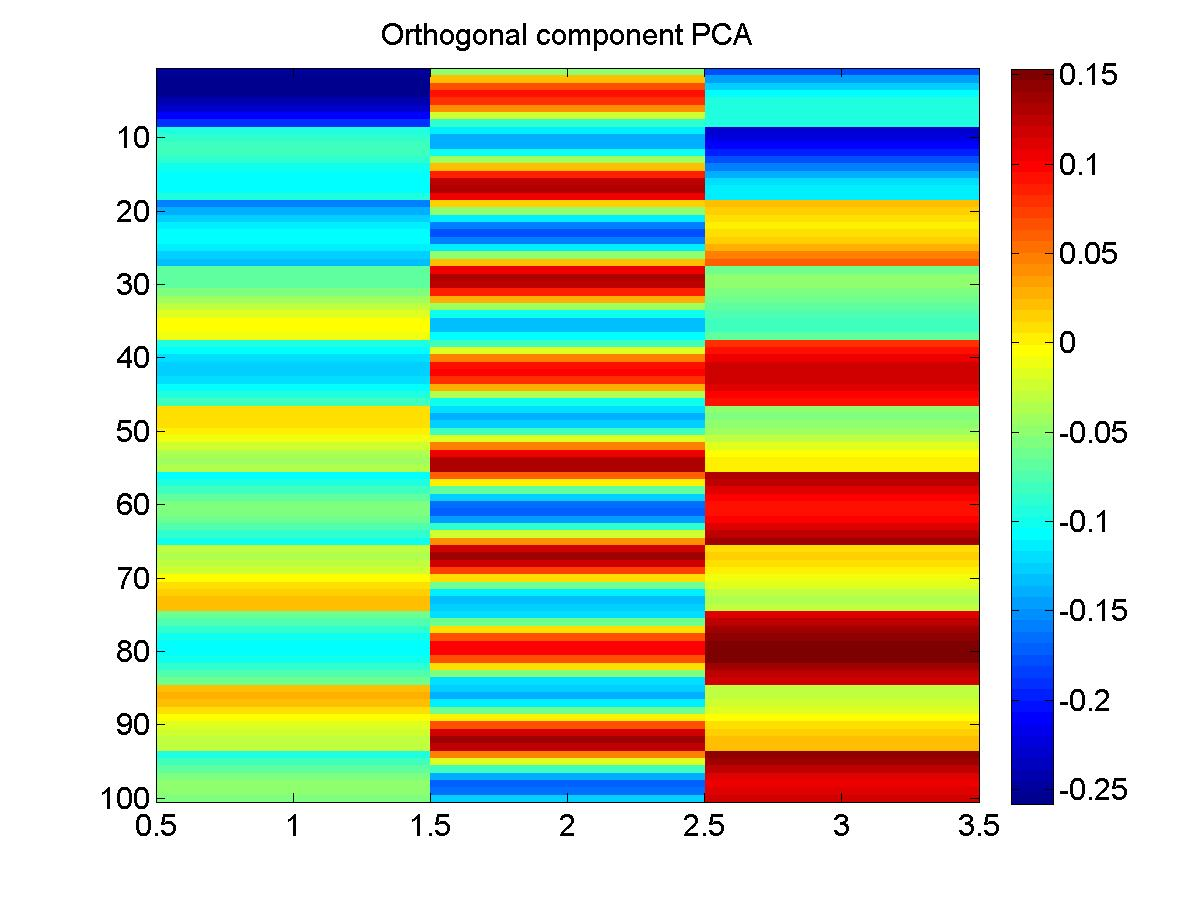
\includegraphics[width=1\linewidth]{204.jpg}
\subcaption{Equivalent of A}\label{EA}
\endminipage\hfill
\minipage{0.33\textwidth}%
\centering
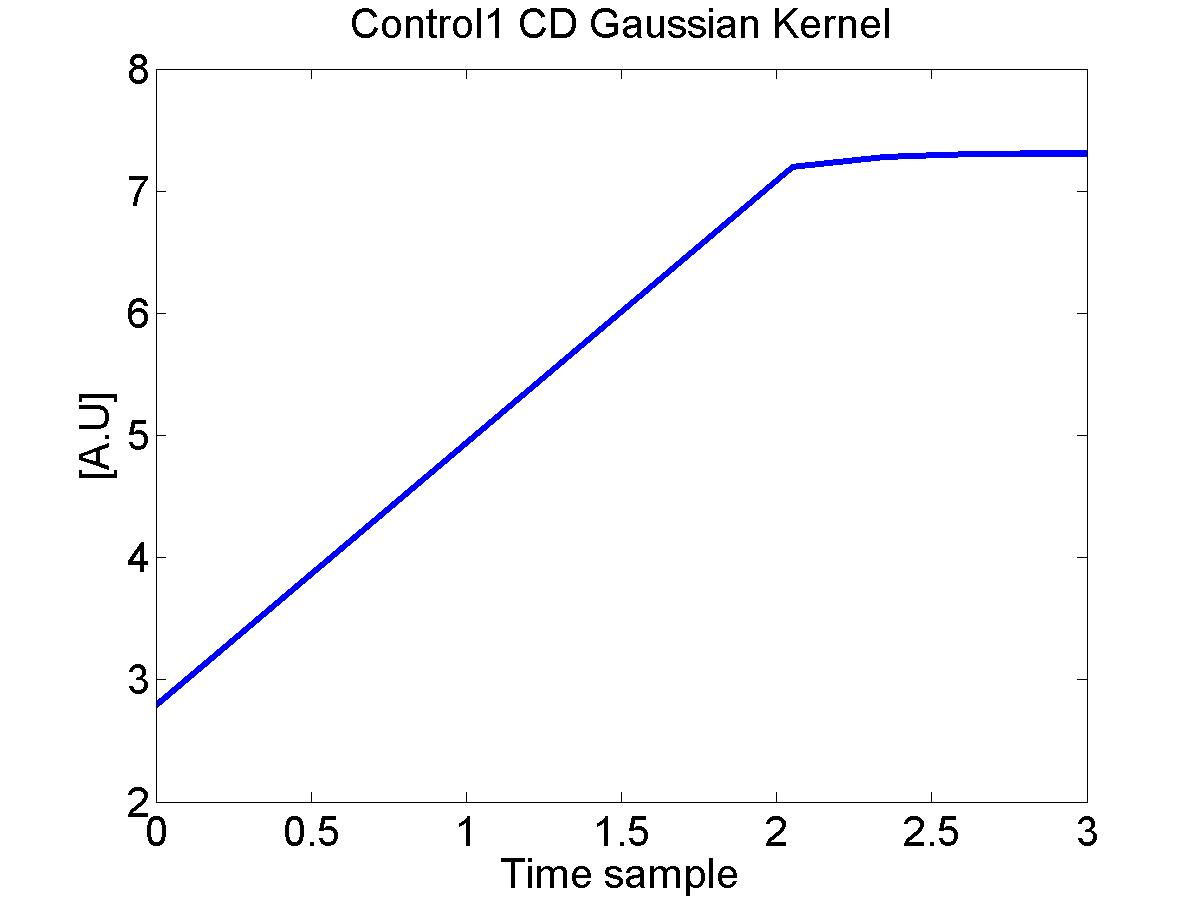
\includegraphics[width=1\linewidth]{205.jpg}
\subcaption{Equivalent of C}\label{EB}
\endminipage\hfill
\minipage{0.33\textwidth}%
\centering
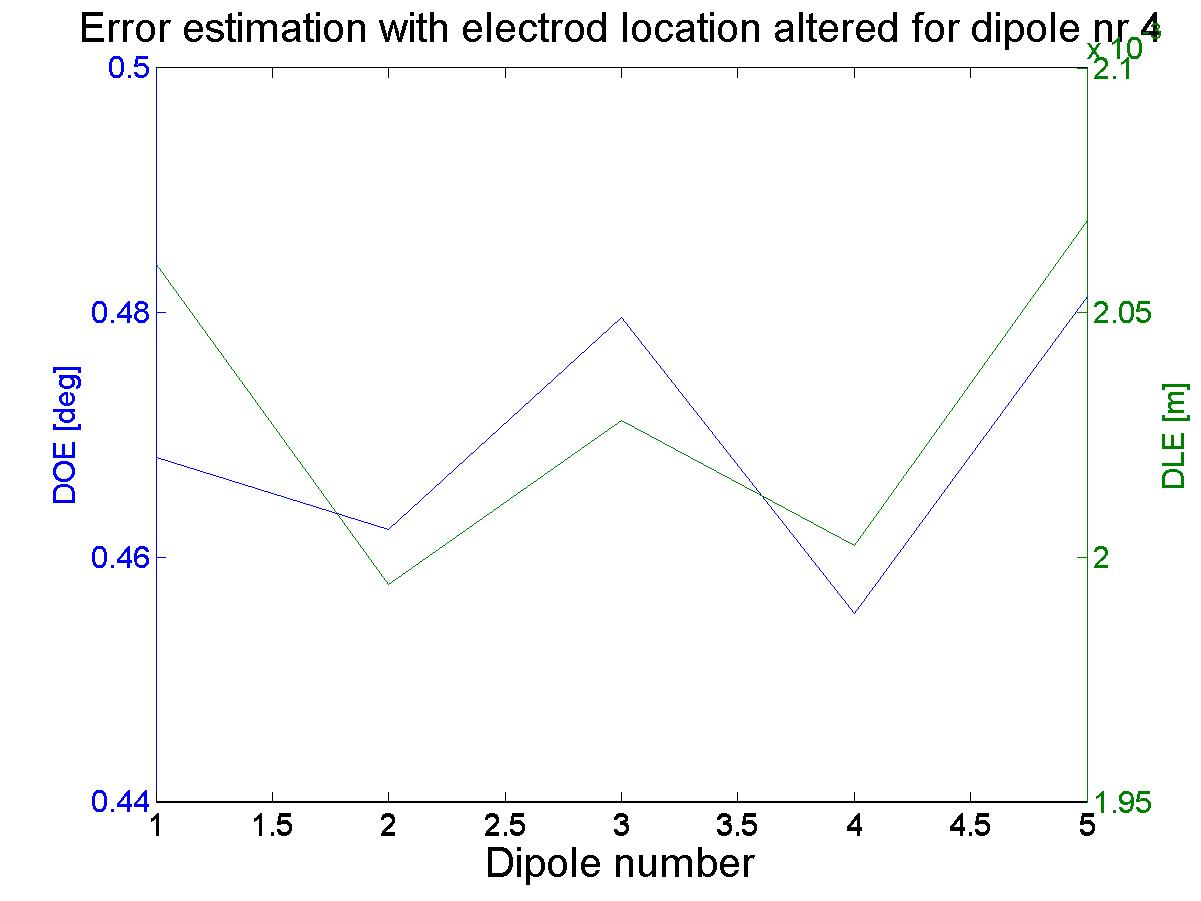
\includegraphics[width=1\linewidth]{206.jpg}
\subcaption{Equivalent of C}\label{EC}
\endminipage\hfill
\caption{PCA decompostion}
\end{figure}

\begin{figure}[!htbp]
\minipage{0.5\textwidth}%
\centering
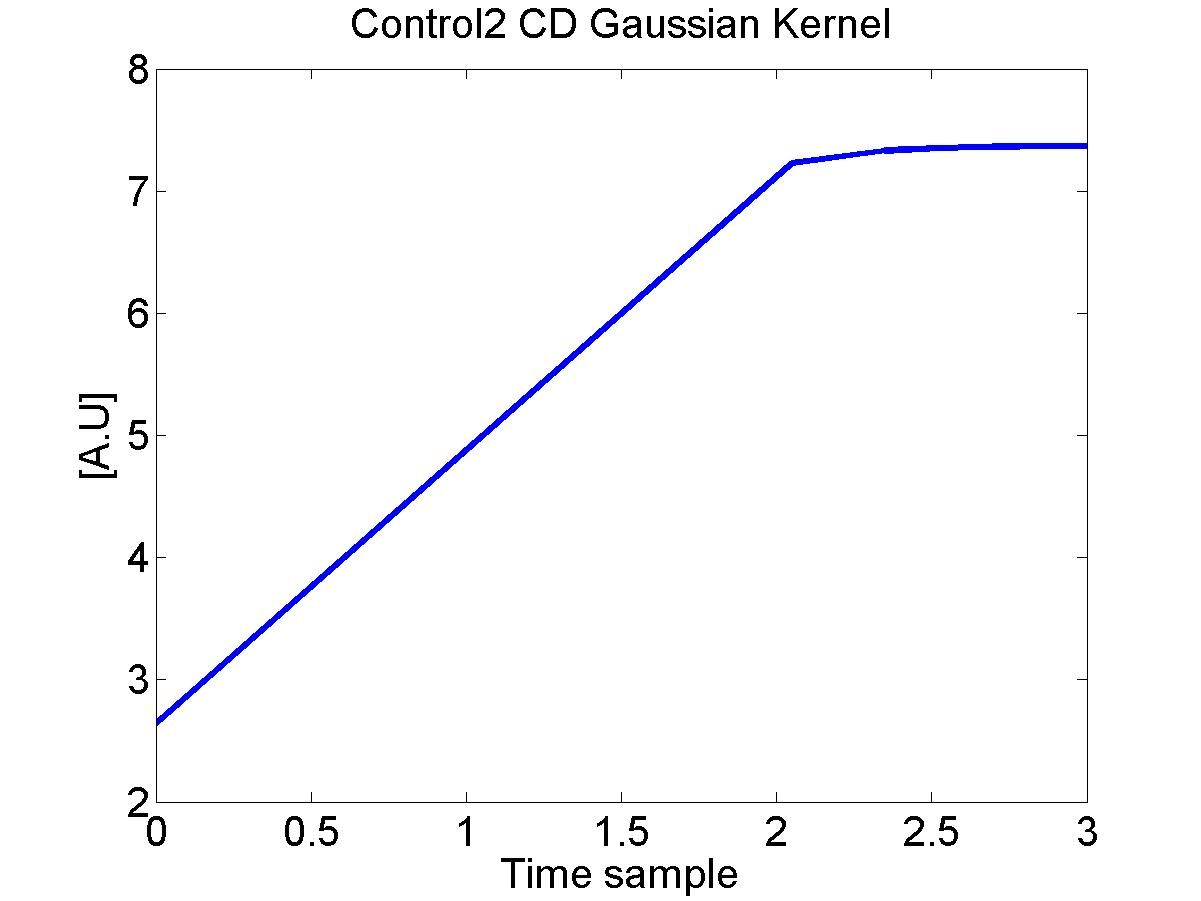
\includegraphics[width=1\linewidth]{207.jpg}
\subcaption{Equivalent of A}
\endminipage\hfill
\minipage{0.5\textwidth}%
\centering
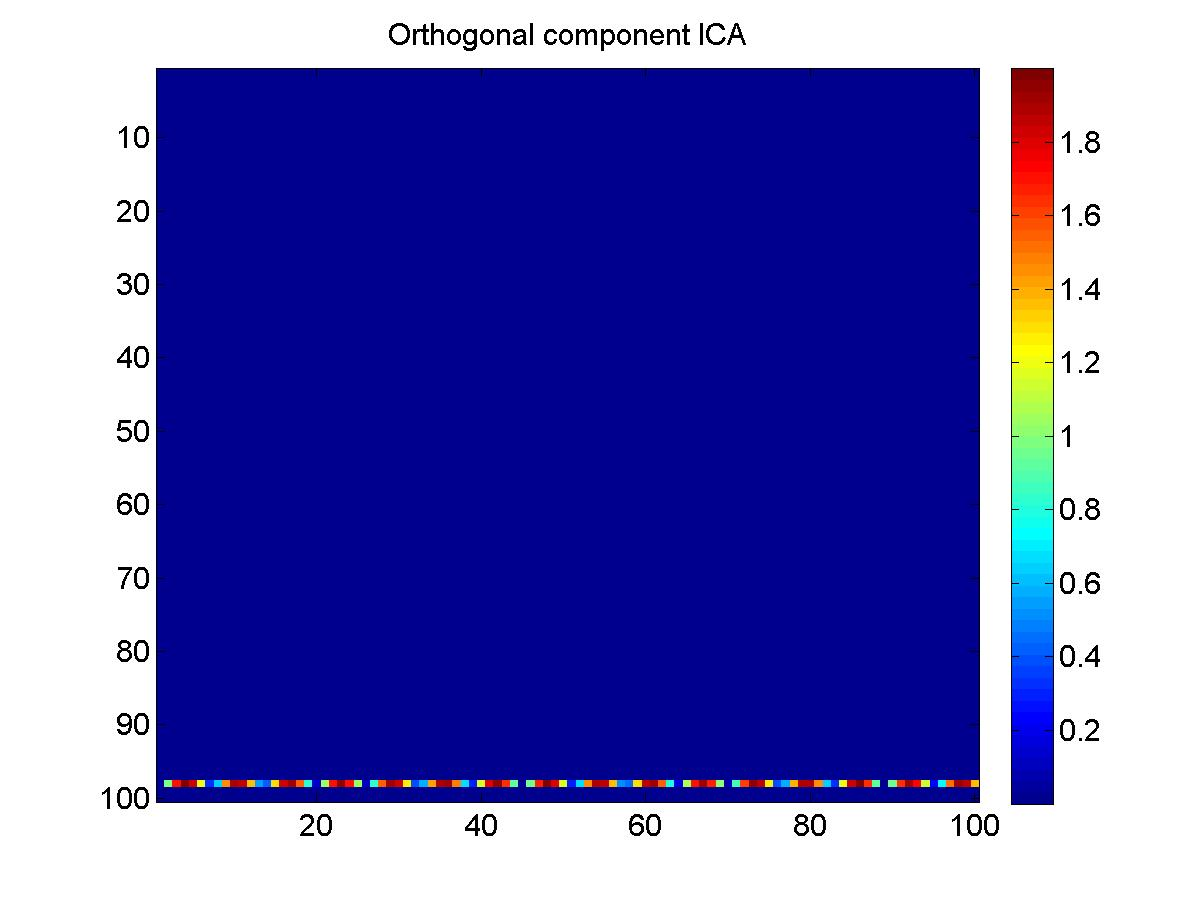
\includegraphics[width=1\linewidth]{208.jpg}
\subcaption{Equivalent of B}
\endminipage\hfill
\caption{ICA decomposition}\label{ICA_E}
\end{figure}

Adding noise at with SNR level of 15dB will compromise the data. This is also noted when multilinear SVD is computed over the new noisy tensor. After computing the Frobenius norm along the each direction it could be noted that the last norm is higher that its equivalent value in the noiseless case in figure \ref{MLSVD2} and \ref{MLSVD1} respectively. Level of noise accommodated into this multilinear subspace will therefore be higher compare the noisy and the noisyless tensor. .  


\begin{figure}[!htbp]
\minipage{0.5\textwidth}%
\centering
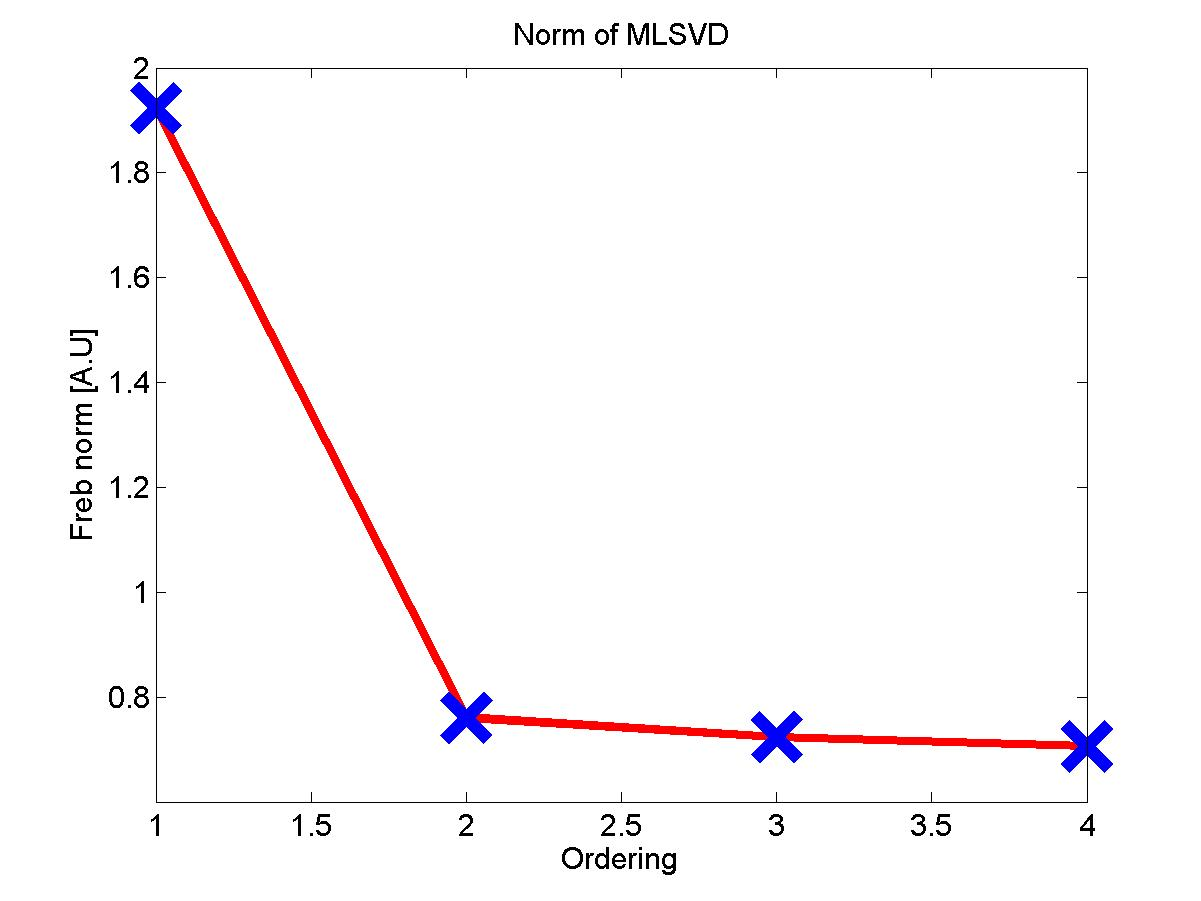
\includegraphics[width=1\linewidth]{209.jpg}
\subcaption{MLSVD norms from the written functions}\label{MLSVD}
\endminipage\hfill
\minipage{0.5\textwidth}%
\centering
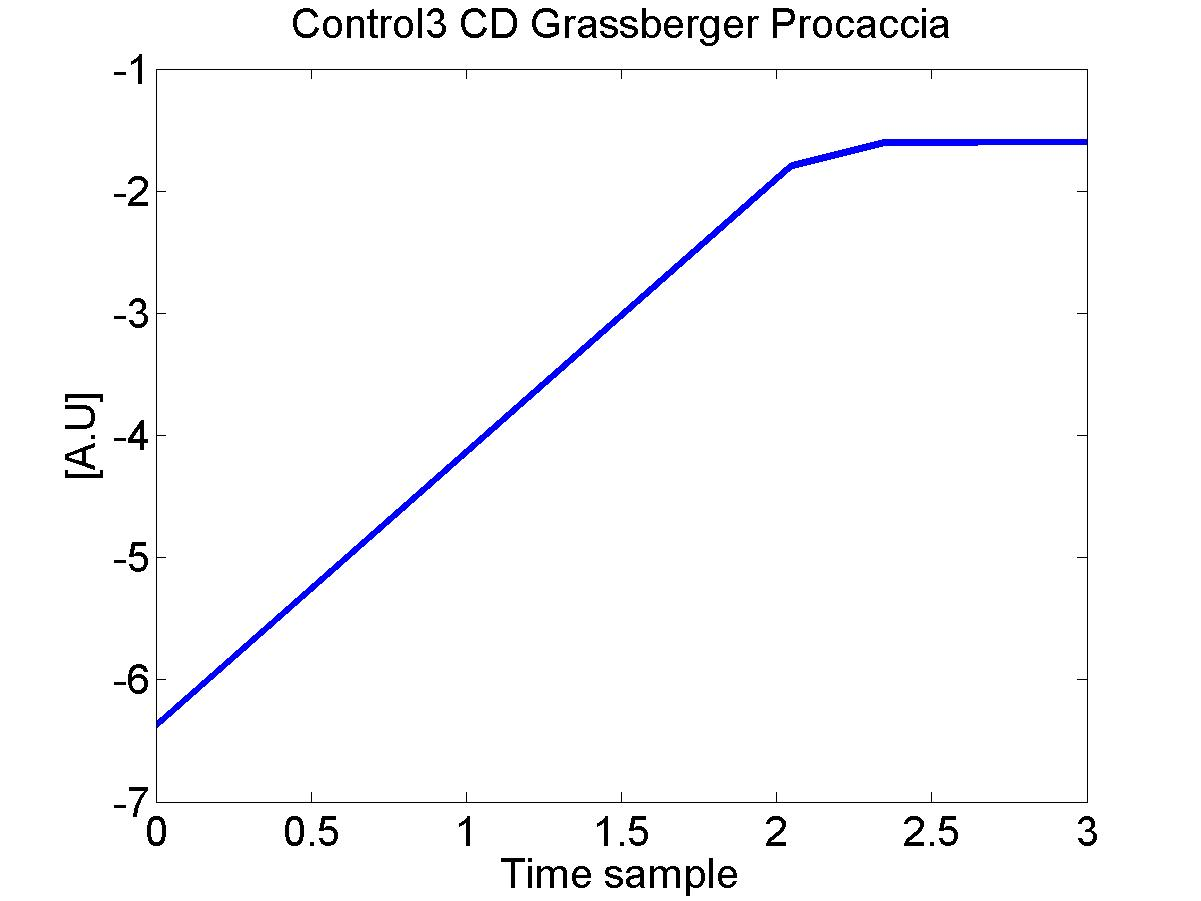
\includegraphics[width=1\linewidth]{210.jpg}
\subcaption{CPD over different rank-1}\label{CPD-1}
\endminipage\hfill
\caption{MLSVD and CPD from the written function}\label{ICA_E}
\end{figure}

\begin{figure}[!htbp]
\minipage{0.5\textwidth}%
\centering
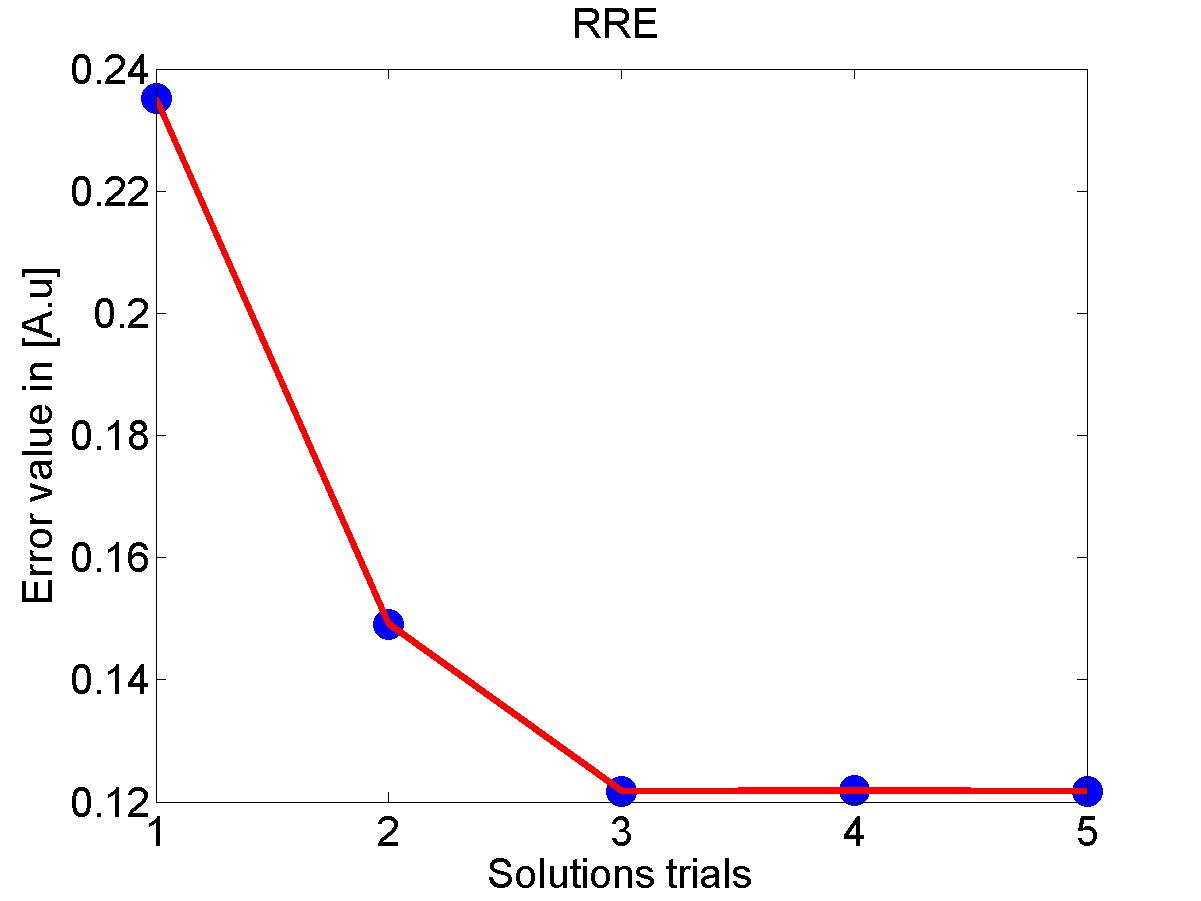
\includegraphics[width=1\linewidth]{211.jpg}
\subcaption{MLSVD norms from tensorlab}\label{MLSVD1}
\endminipage\hfill
\minipage{0.5\textwidth}%
\centering
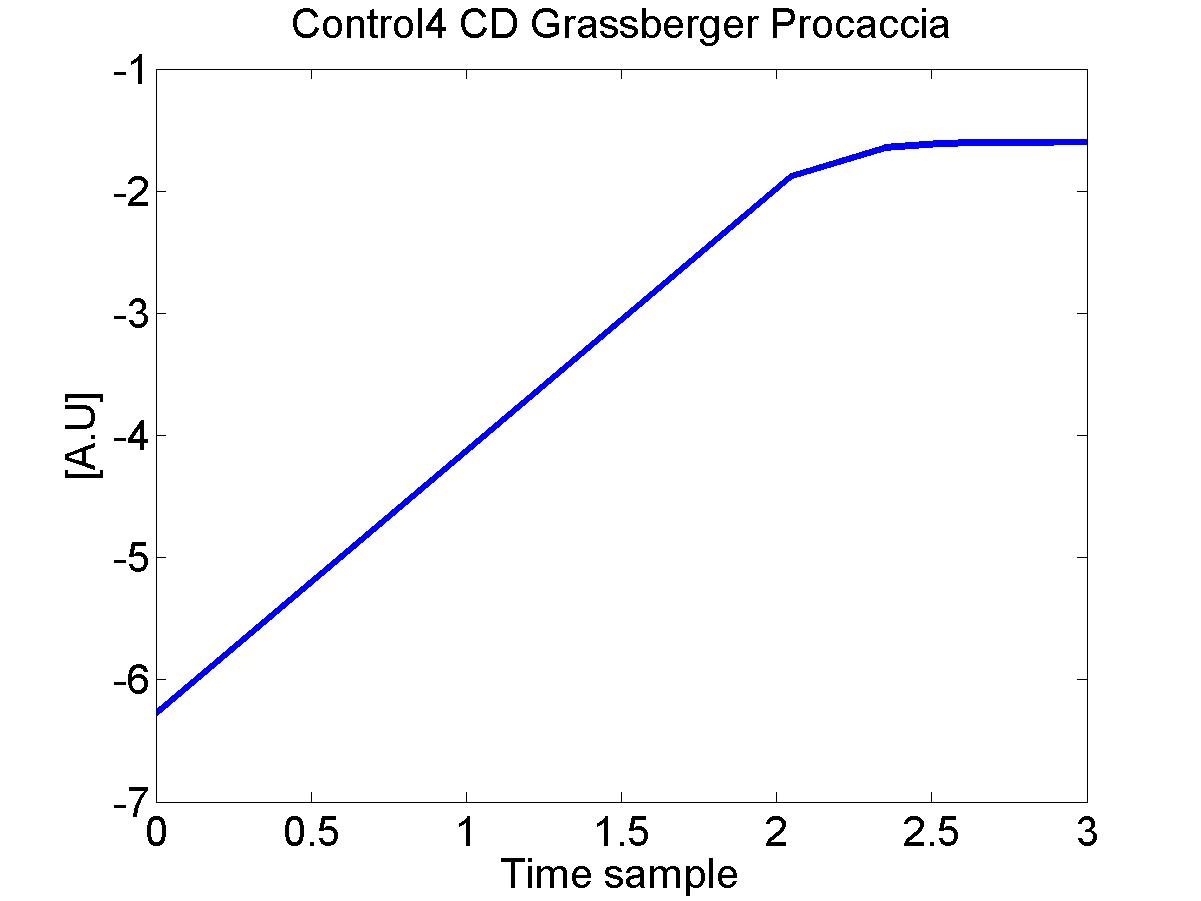
\includegraphics[width=1\linewidth]{212.jpg}
\subcaption{MLSVD norms from tensorlab}\label{MLSVD2}
\endminipage\hfill
\caption{MLSVD via tensorlab}\label{ICA_E}
\end{figure}


Regarding the CPD alternative least square (ALS) has been implemented. Even though this is not the best choice possible due to the main two facts. First the non-stationary of the limit points might lead to a solution that is potentially not the minimum. Secondly the existence of limit points is not guaranteed therefore the convergence might not even happen \cite{5}.

Nevertheless it was still decided to implement ALS since its outcome was fairly convincing. In the figure below are the result of the Frobenius norm for different rank-1 tensor decompositions \ref{CPD-1}. 

Even though the norm of each estimation is low ALS tends not to converge better as the number of rank-1 tensors increases which could be seen in figure \ref{CPD-1}.

Alternatively Nonlinear Least Square NLS CPD has been utilized from tensorlab. Wherein via CPD-NLS multiple initialization are used therefore any local optima is avoided in this case. In order to reach the best estimation possible the the stop criteria is put at the order of -20. This will enable a very slow error to be toleration. Further more pseudo-random initialization are used in order explore are more heterogeneous space as possible. 

\begin{figure}[!htbp]
\centering
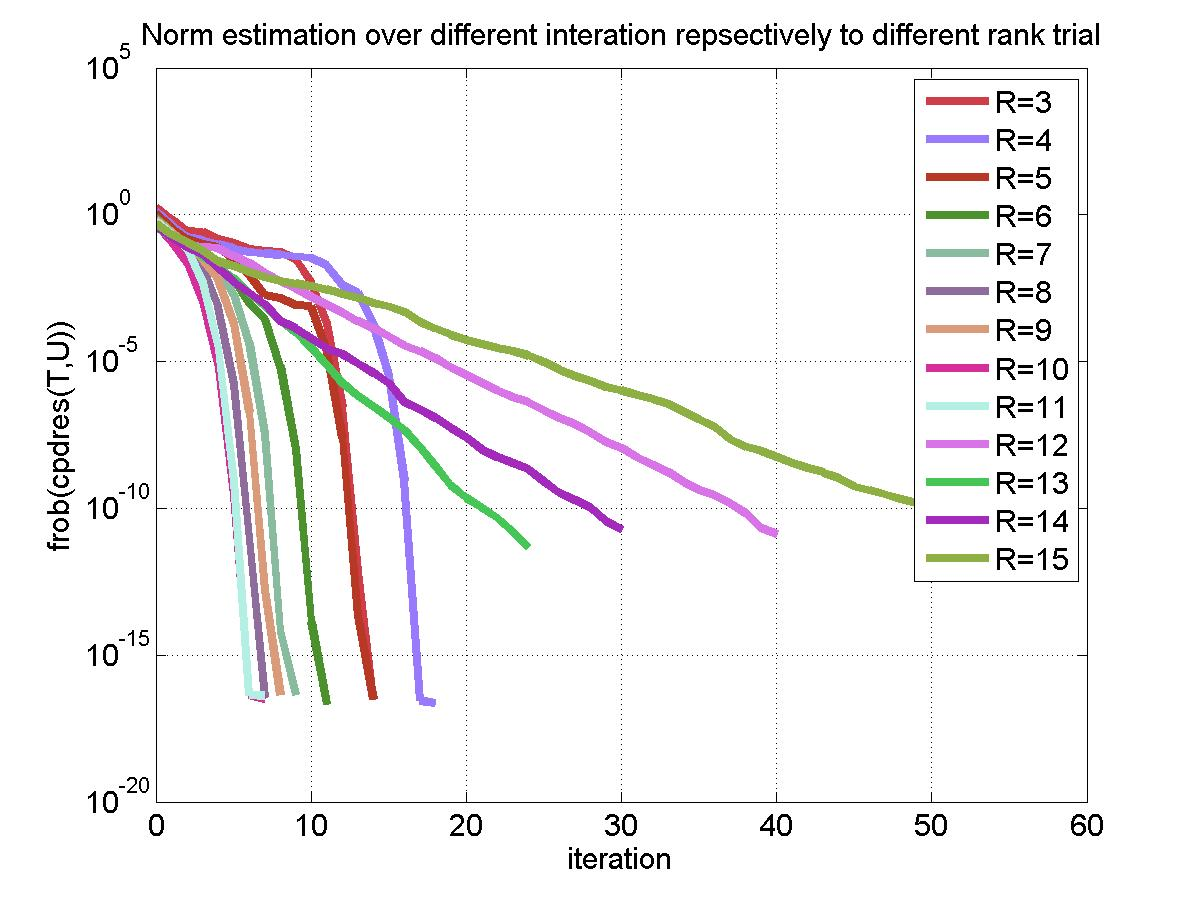
\includegraphics[width=0.5\linewidth]{213.jpg}
\caption{CPD performance using tensorlab}
\end{figure}


 CPD performs fairly good at rank close to 11 where from the figure \ref{CPD-2} meaning that high number of iteration is needed to reach the stopping criteria at CPD with rank 12,13,14. Whereby we could estimated that the rank of the noisy tensor is 11. Additionally, as the trial rank number goes higher than 11, the number of iteration required to reach the stopping criteria tends to be higher. 
